%#########################################
% For 140601 GitHub Kaigi
% title: GitHubで行うreproducible research
%#########################################
\documentclass[dvipdfmx, 14pt]{beamer}
\usepackage{pxjahyper, otf, mediabb, tikz, wrapfig}
\usepackage{pifont}
\usetheme{default}
\renewcommand{\kanjifamilydefault}{\gtdefault}
\renewcommand{\familydefault}{\sfdefault} % 欧文書体をHelveticaに
\setbeamertemplate{navigation symbols}{}

\setbeamertemplate{background canvas}{
\includegraphics[height=\paperheight]{bg}}


\setbeamerfont{title}{size=\huge, series=\bf}
\setbeamercolor{title}{fg=black}
\setbeamercolor{normal text}{fg=black, bg=custom.bgc}
\setbeamercolor{frametitle}{fg=black}

\definecolor{custom.fc}{HTML}{F4F6F7}
\definecolor{custom.bgc}{HTML}{4798DD}

\graphicspath{{../../src/}}

%#######*****####### titile #######*****#######***
\title{GitHubで行う\\reproducible research}
\author[瓜生]{\href{http://urush.postach.io}{瓜生真也}}
\institute[横国大院・環情]{横浜国立大学大学院 環境情報学府}
\subject{LT slide for GitHubKaigi@Shibuya}
\date{\scriptsize GitHub Kaigi(@Shibuya), June 1, 2014

\vspace{1em}
\href{http://github.com/uribo/rep-res-guideline}{github.com/uribo}

%\vspace{0.5em}
%\href{http://github.com/uribo/rep-res-guideline}{Repository is here.}
}
%\logo{
\includegraphics[height=0.8cm]{RR-icon}\hspace{15pt}\vspace{230pt}}

%#######*****#######*****#######*****#######***
\begin{document}
\frame{
  \begin{center}
  \Huge 論文
  \end{center}}

{\usebackgroundtemplate{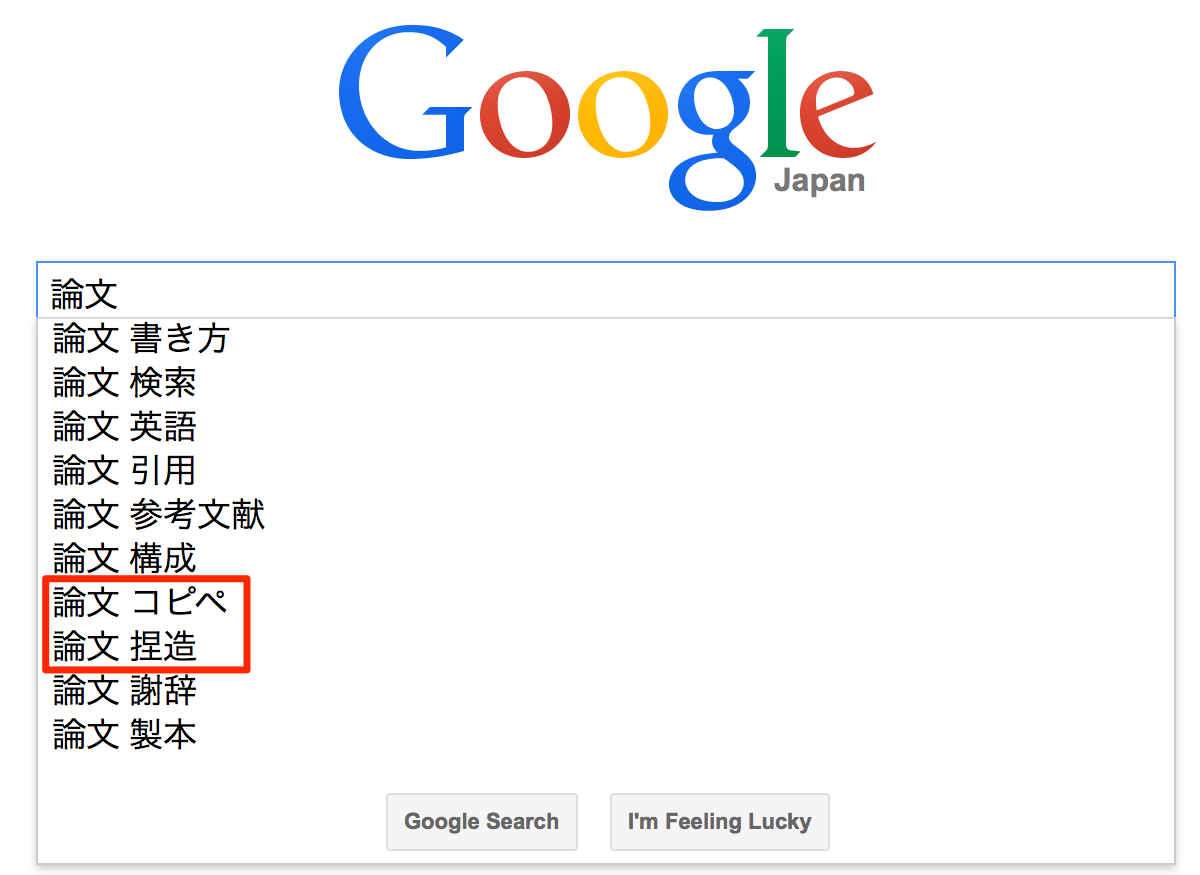
\includegraphics[width=\paperwidth]{gg-suggest}}%
\frame{}}%なぜ論文に再現性が必要なのか

{\usebackgroundtemplate{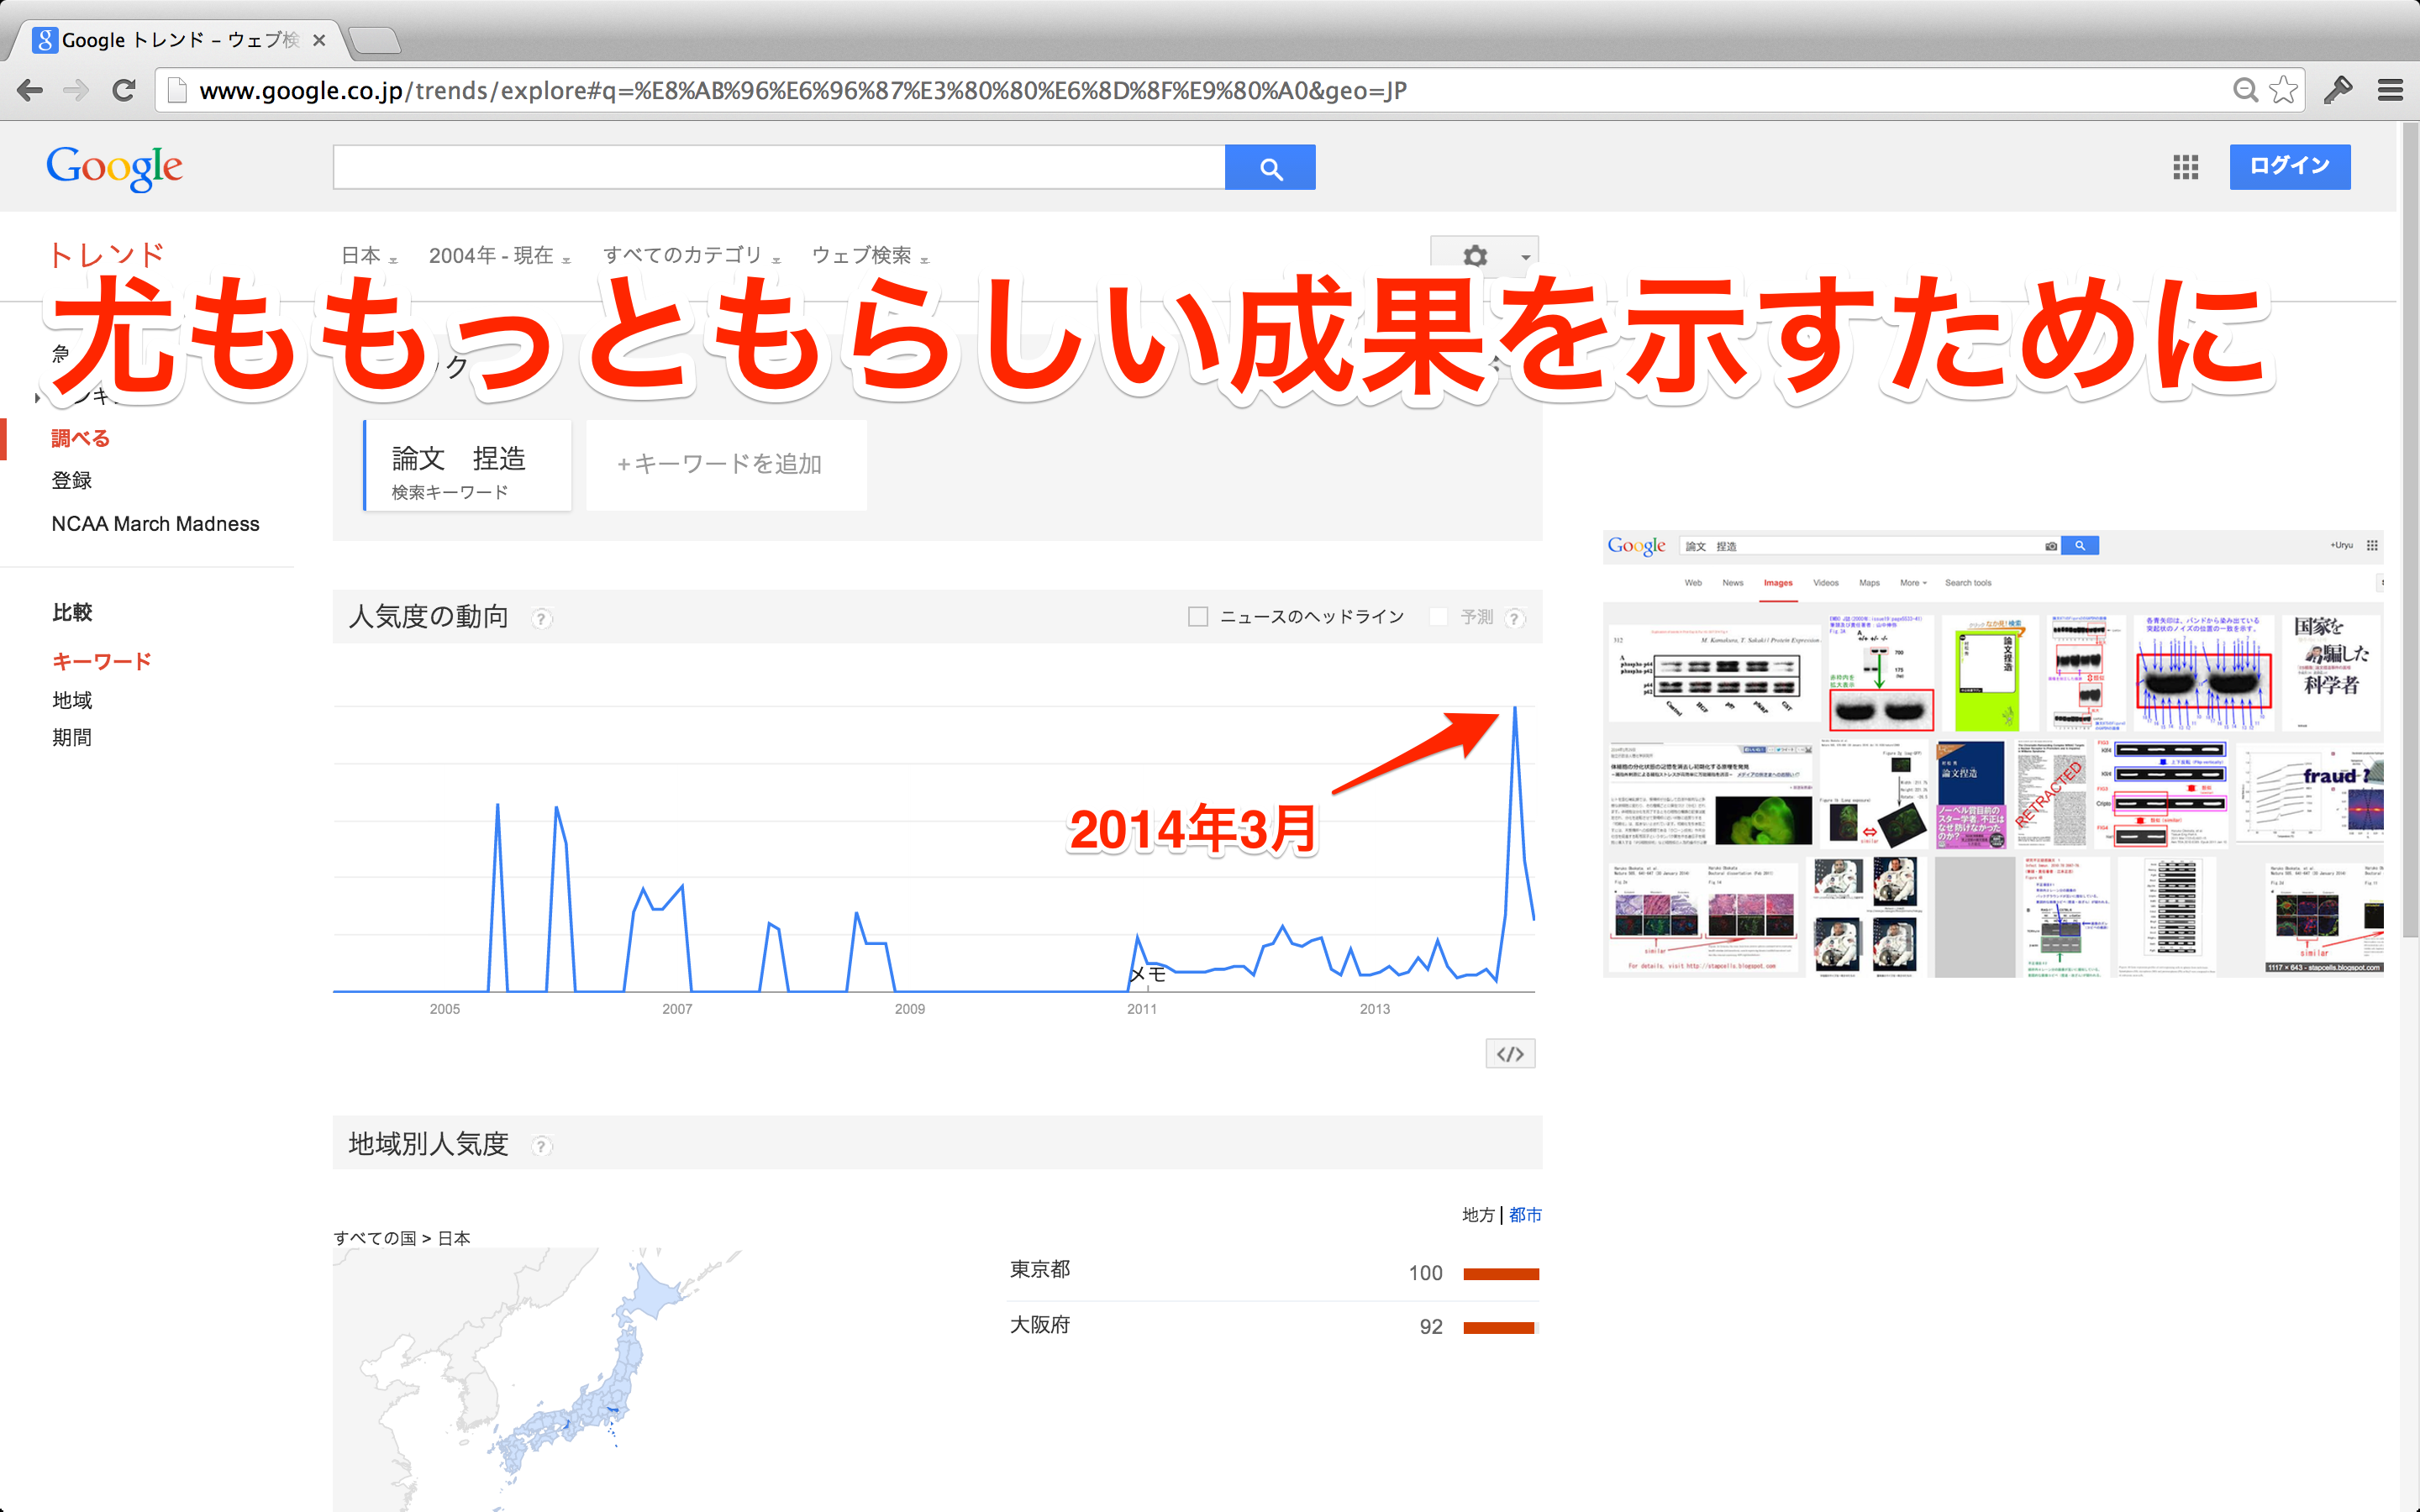
\includegraphics[width=\paperwidth]{gg-trends}}%
\frame{}}%尤ももっともらしい成果を示すために

\frame{
\frametitle{Reproducible Research (RR)}
  {\Large 再現可能な研究}\\
  \vspace{0.5em}
  論文に書かれている方法、条件で行えば、\\同様の結果が得られる
  \begin{wrapfigure}{o}[60pt]{60mm}
    
\includegraphics[height=3.5cm]{RR-icon}
  \end{wrapfigure}
  \vspace{0.5em}
  \begin{itemize}
  \setlength{\itemindent}{2em}
  {\Large
    \item[\ding{51}] 客観性
    \item[\ding{51}] 明瞭性
    \item[\ding{51}] 妥当性
  }\end{itemize}
  \vspace{0.5em}
  %{\small ...GitHubを活用したRRの実践方法を提案}
  }

\frame{\titlepage}
%#######*****#######*****#######*****#######***
\frame{
  \frametitle{研究の流れ}
  統計解析と論文の執筆は鬼門
  \begin{center}
  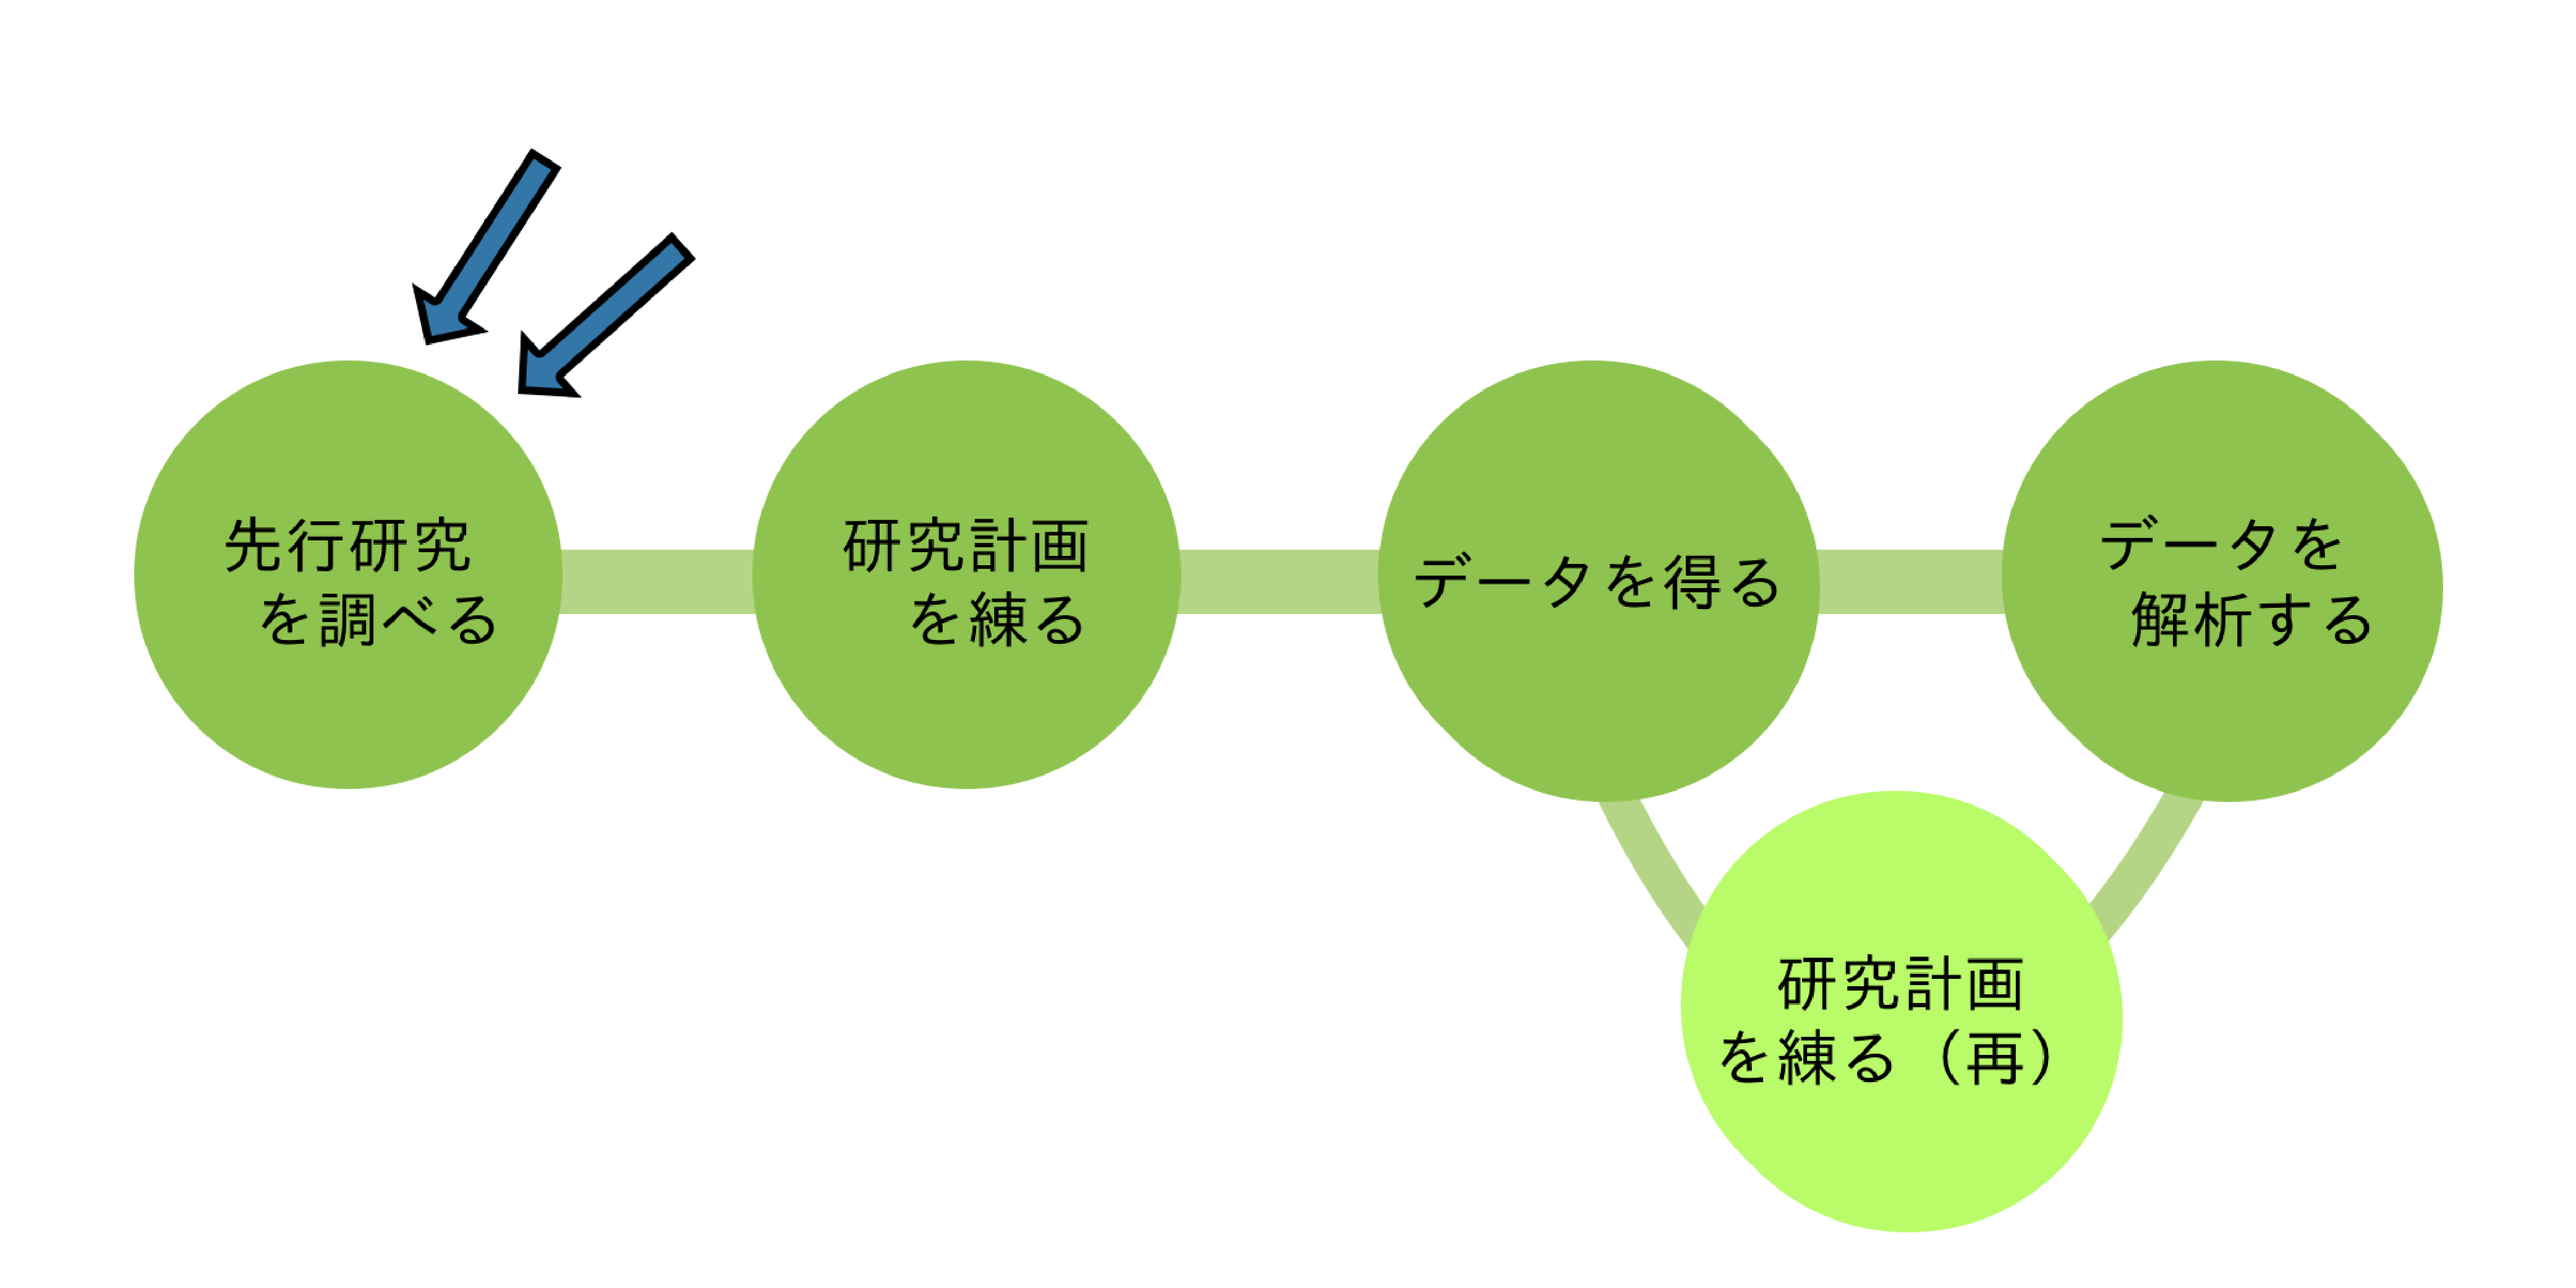
\includegraphics[width=11cm]{research-flow}
  \end{center}
}

{\usebackgroundtemplate{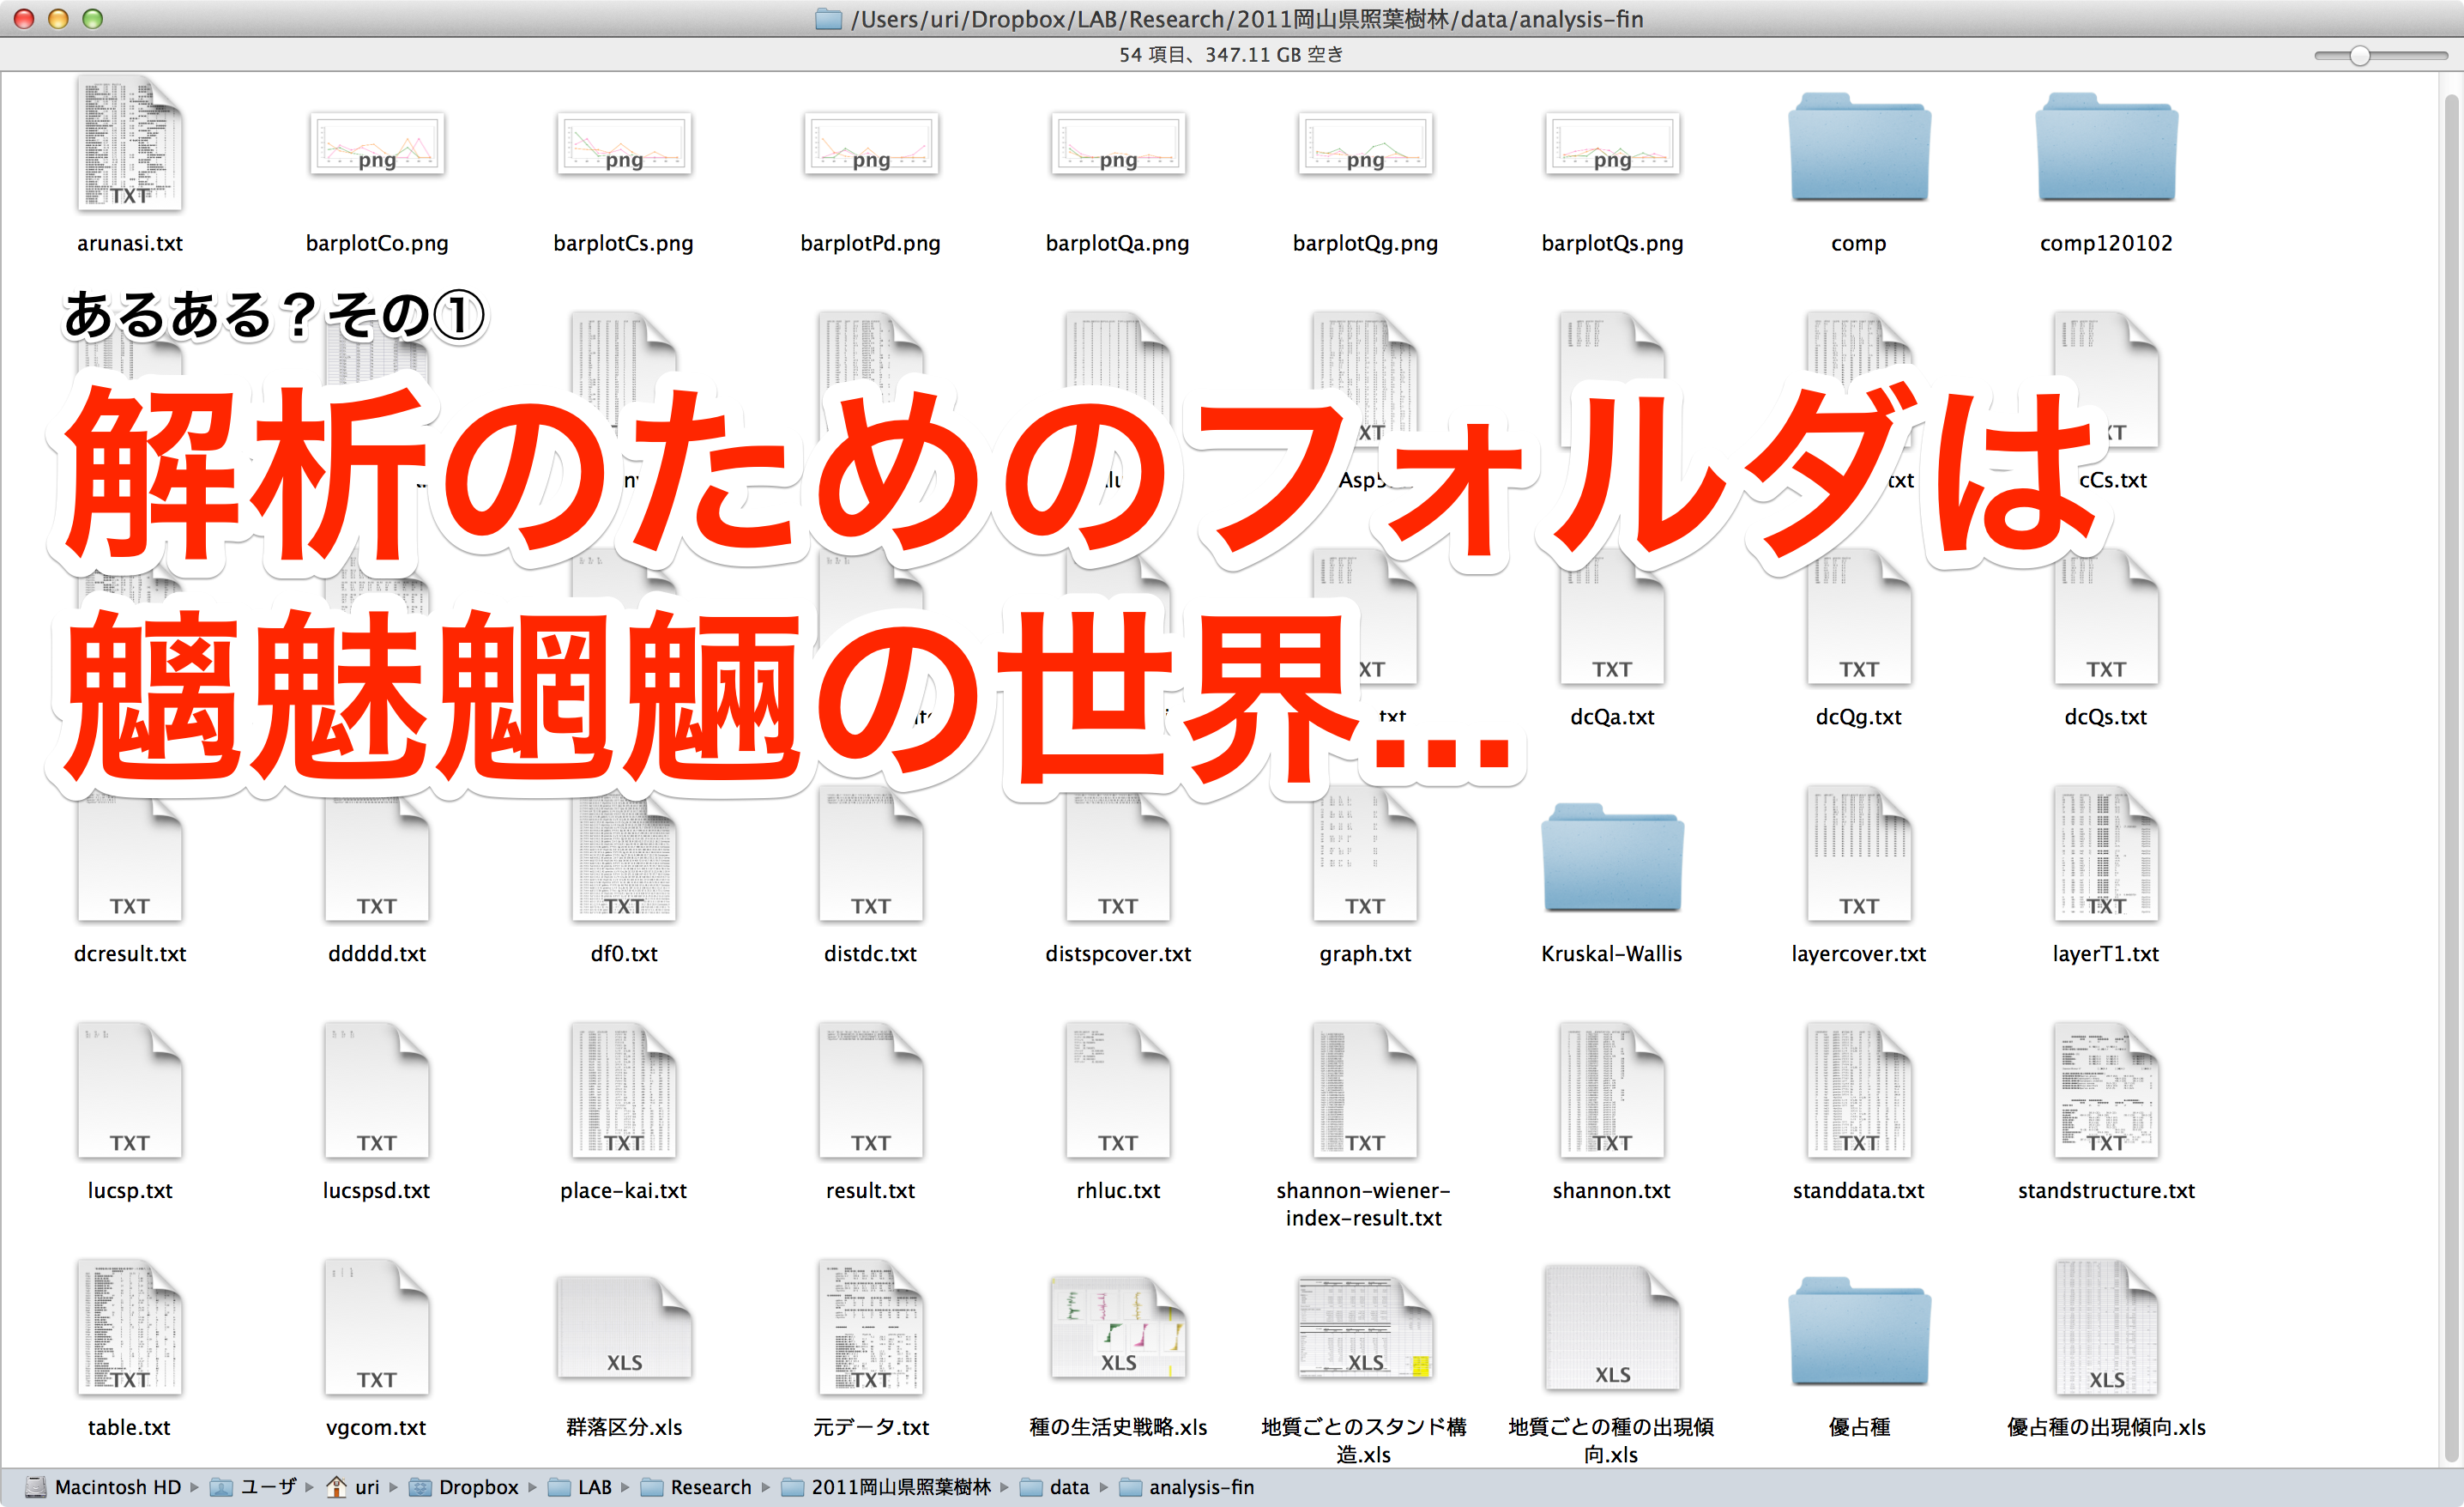
\includegraphics[width=\paperwidth]{misc-files}}%
\frame{}} %解析フォルダは魑魅魍魎の世界

{\usebackgroundtemplate{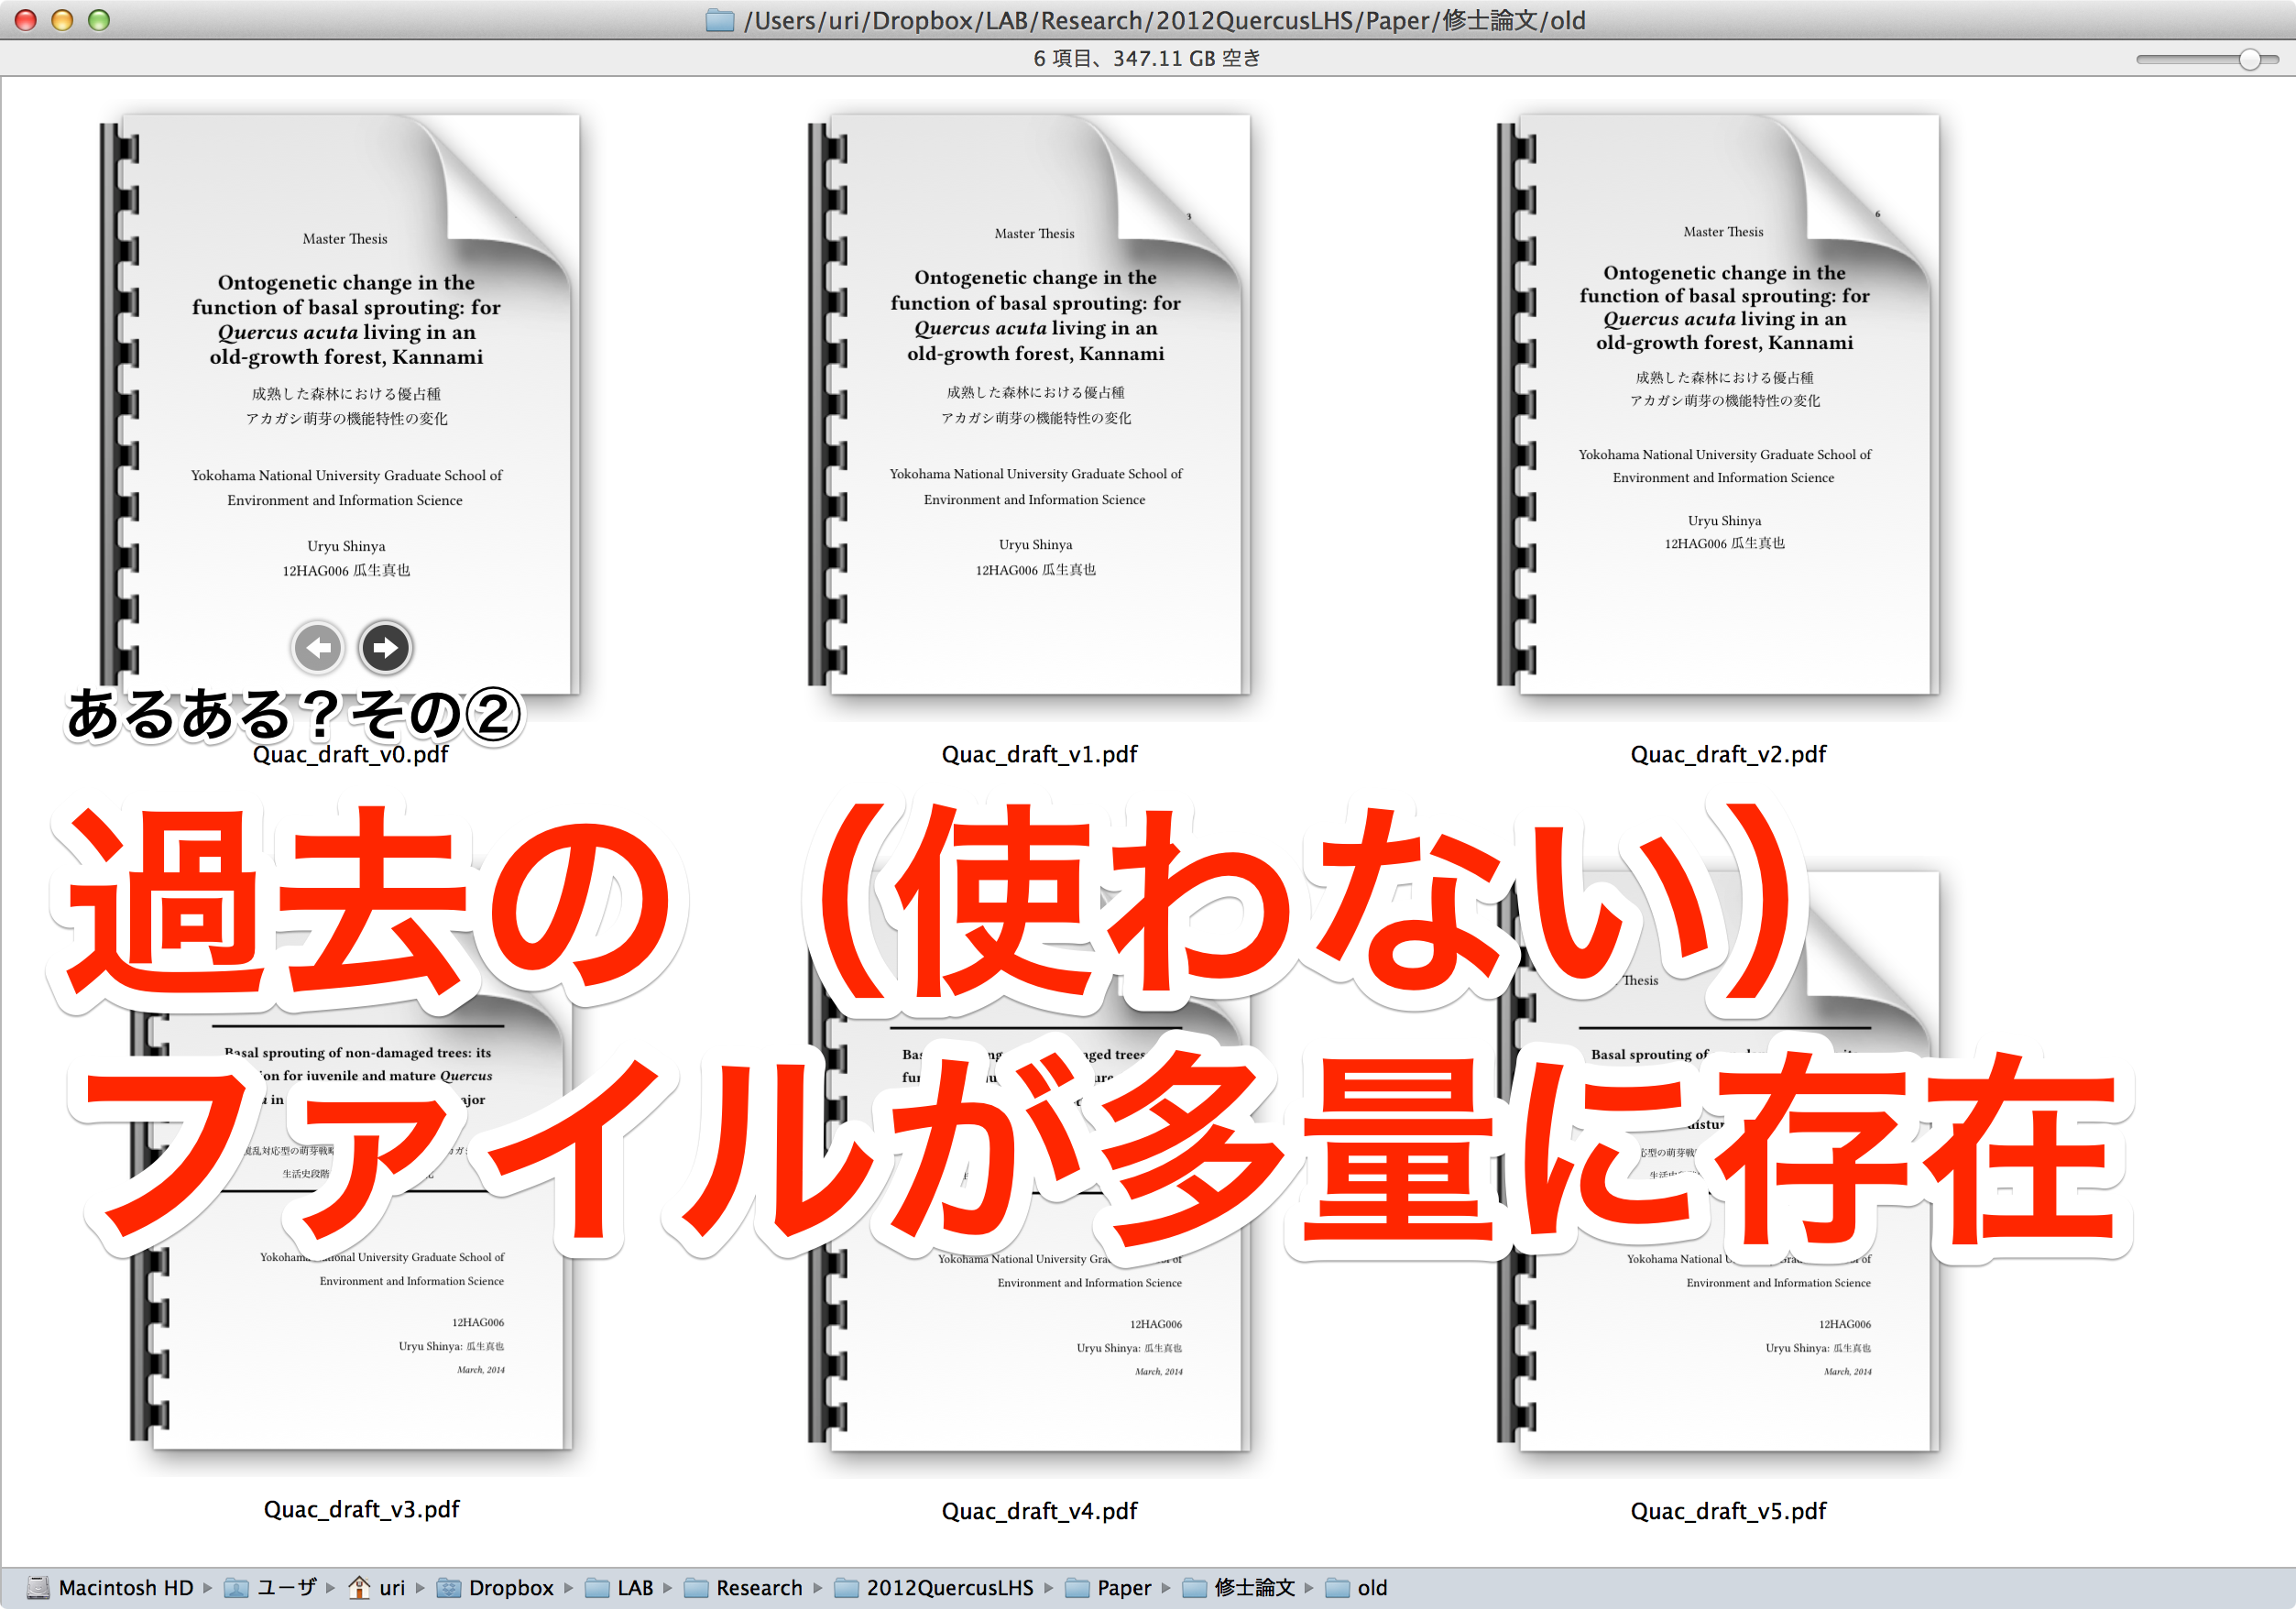
\includegraphics[width=\paperwidth]{old-files-collection}}%
\frame{}} %過去のファイル

\frame{
  \frametitle{Git/GitHubの特徴を活かした\\研究のススメ方}
  \vspace{-2.6em}
  \begin{center}
  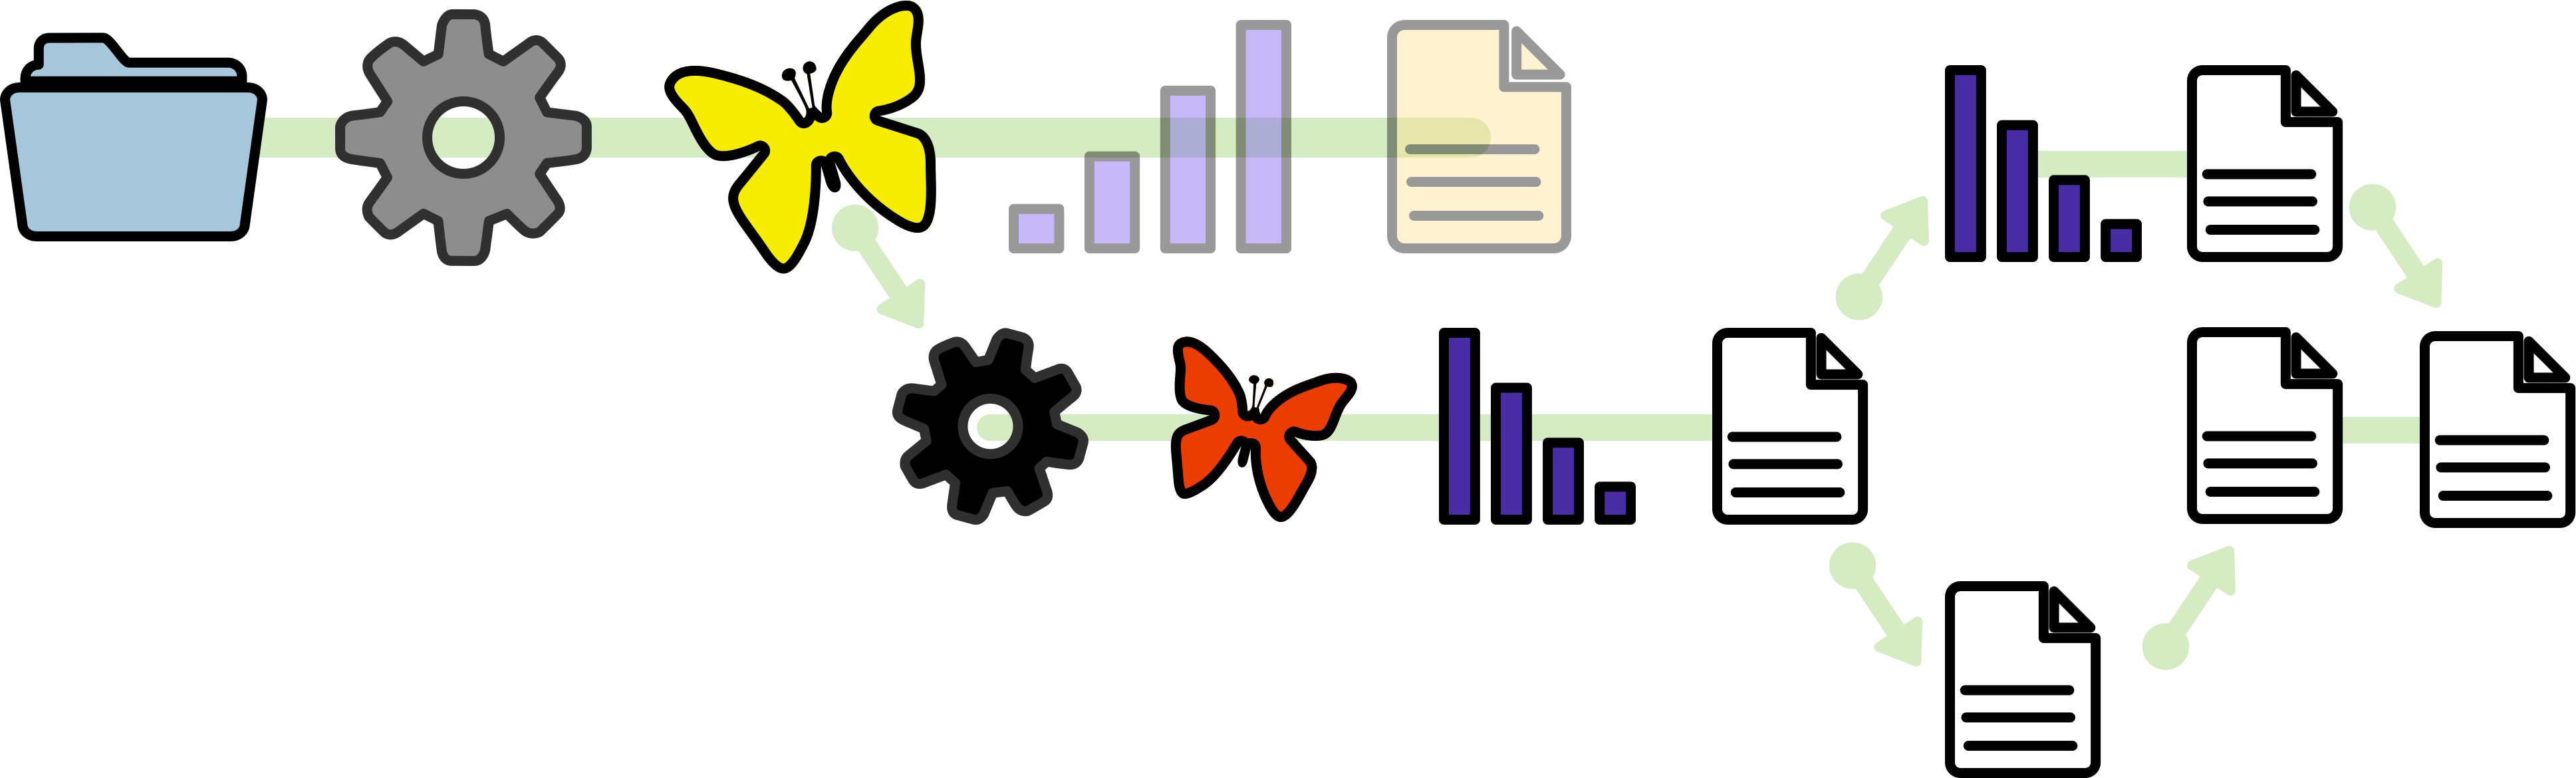
\includegraphics[height=3cm]{research-flow-branch}
  \end{center}
  \vspace{-1em}
  \begin{itemize}
    \item バージョン管理システム{\small (リポジトリ、ブランチ)}
    \item issues
    \item commit
  \end{itemize}
}

%\frame{
%  \frametitle{RRを行う際のガイドライン}
%  \vspace{-1.0em}
%  \begin{center}
%  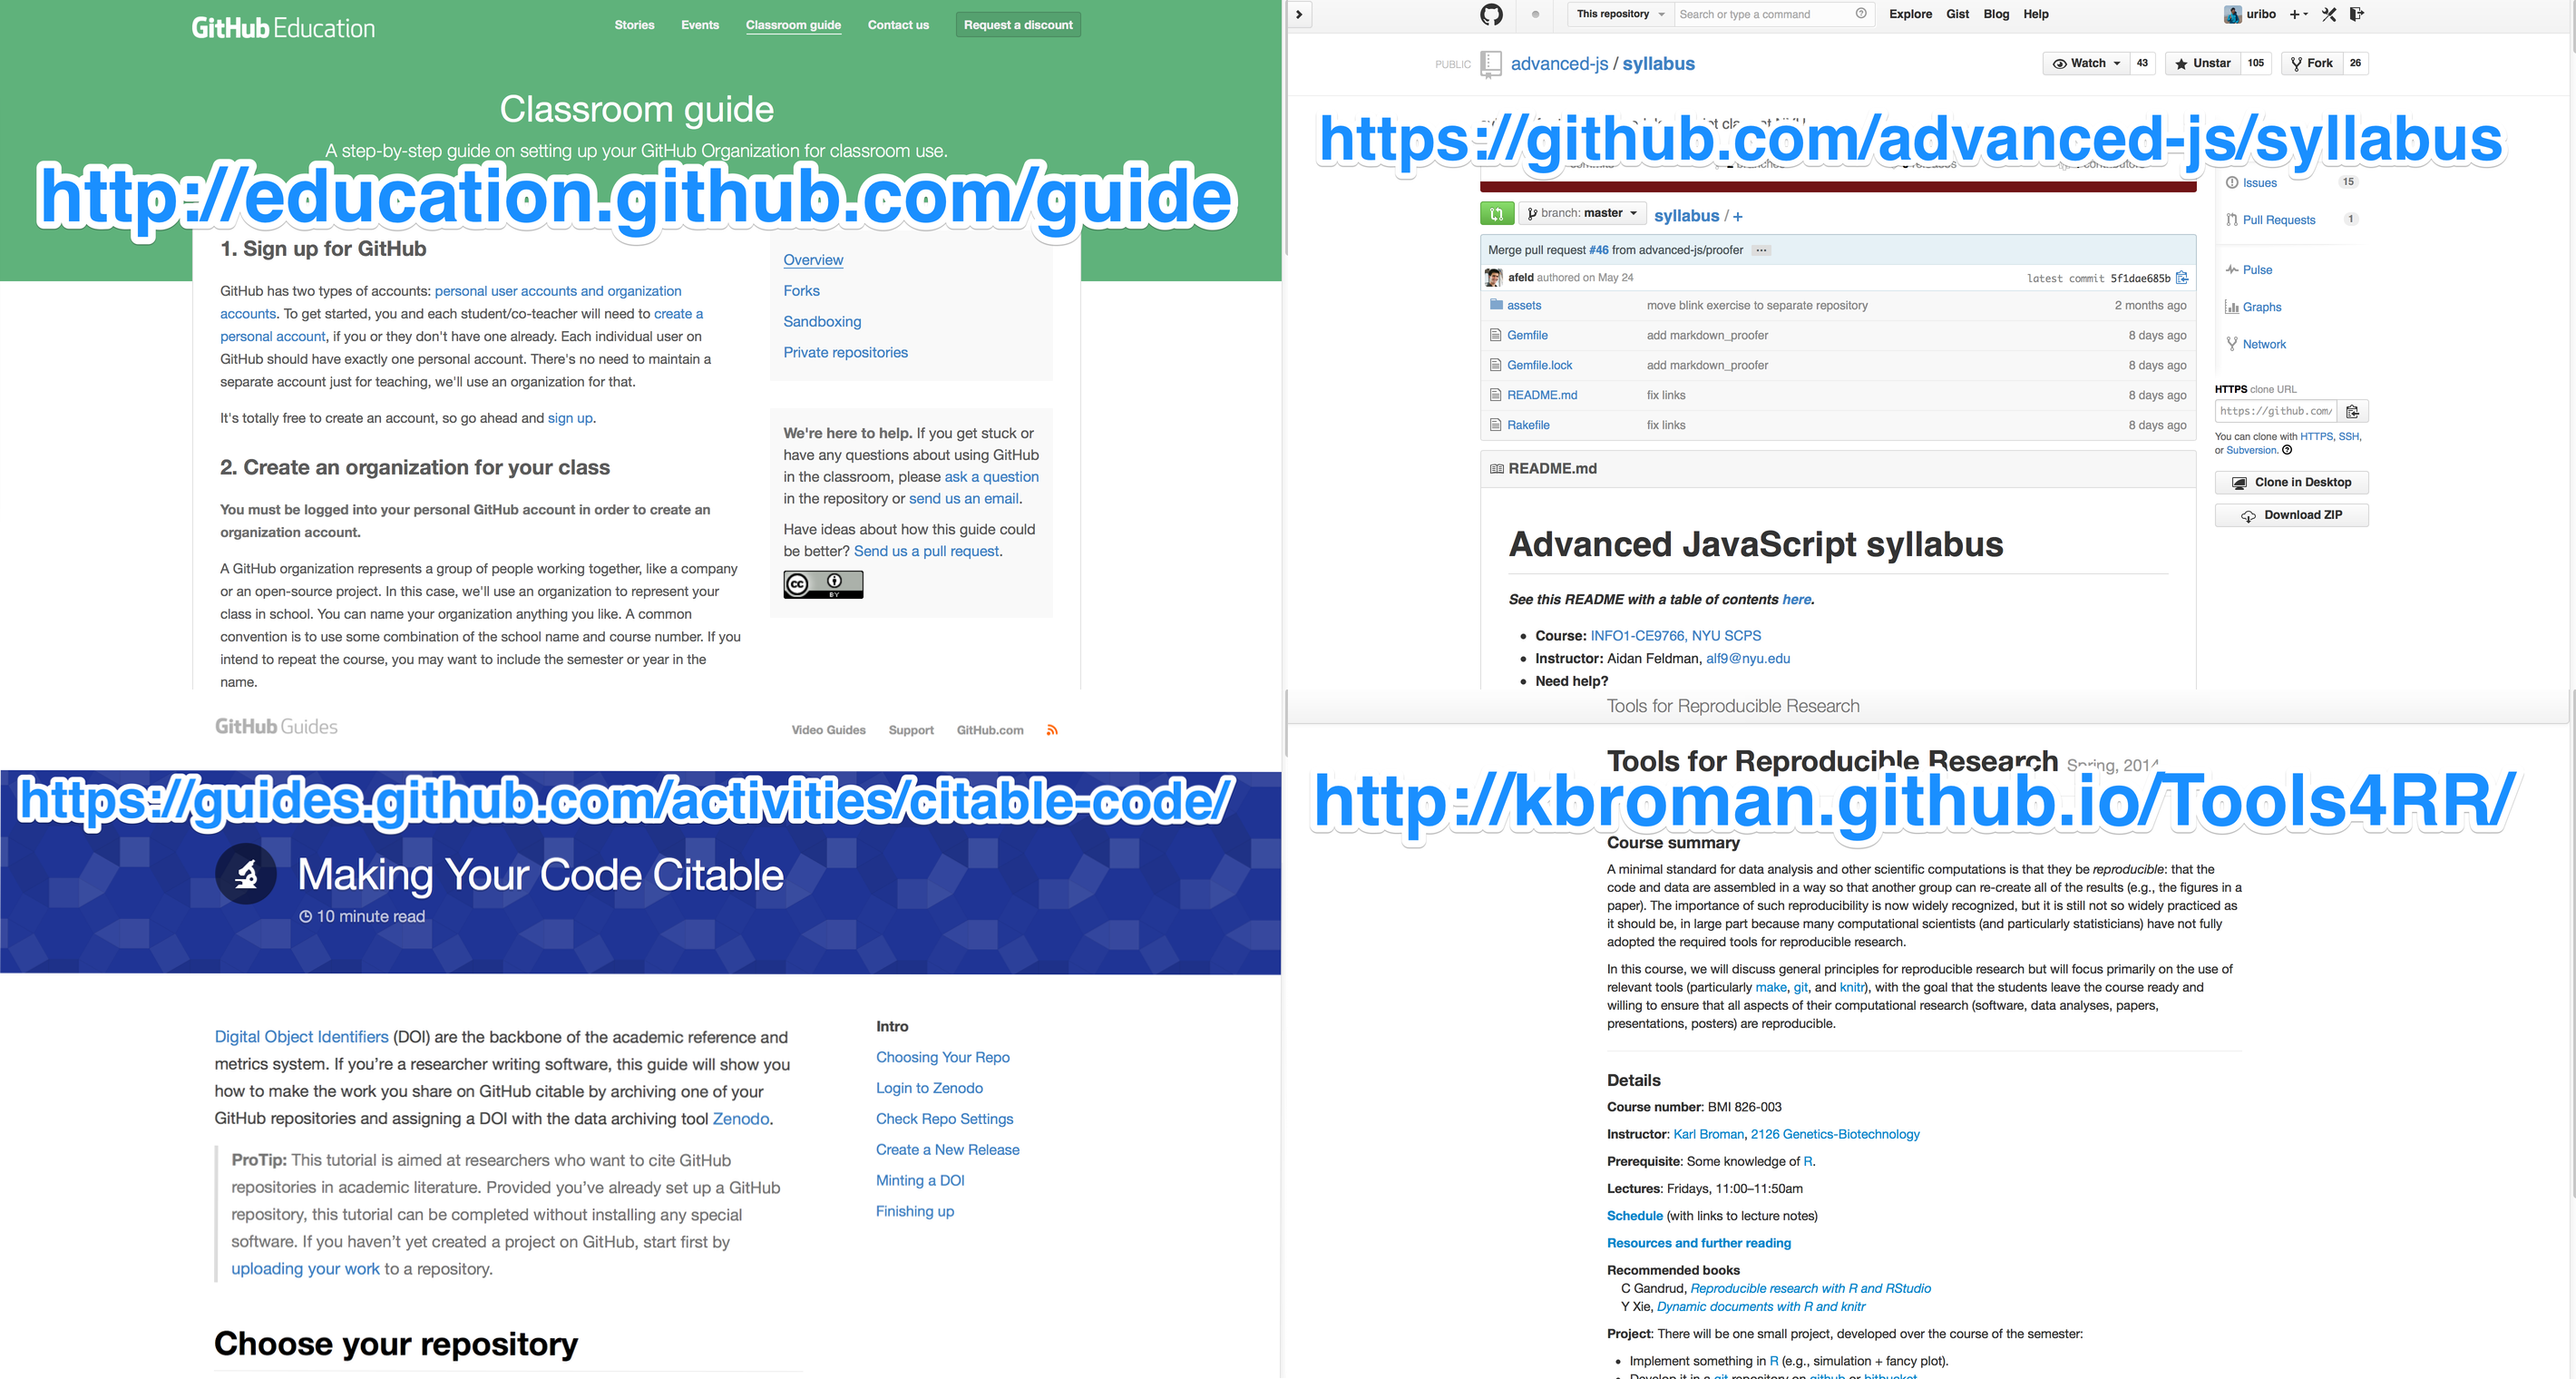
\includegraphics[height=4cm]{course-and-guidelines}\\
%  {\Huge なければ作れば\\いいじゃない}\\
%  言い出しっぺの法則
%  \end{center}
%}

\frame{
  \frametitle{みんな大好きR}
  \begin{center}
  
\includegraphics[height=3cm]{instruction}\\
  \end{center}
}


\frame{
  \frametitle{みんな大好きLaTeX}
  \begin{center}
  
\includegraphics[height=3cm]{latex-logo}\\
  \end{center}
}


\frame{
  \frametitle{著者、出版社、査読者への指示書き}
  \begin{center}
  
\includegraphics[height=3cm]{instruction}\\
  \end{center}
}



\frame{
  \frametitle{今後の展望と課題}

}




\end{document}
